\documentclass[aspectratio=169,10pt]{beamer}

\usetheme{Madrid}
\usecolortheme{default}
\setbeamertemplate{navigation symbols}{}
\setbeamertemplate{footline}[frame number]

\usepackage{booktabs}
\usepackage{graphicx}
\usepackage{tikz}
\usepackage{array}
\usepackage{adjustbox}
\usetikzlibrary{positioning,fit,arrows.meta}

\graphicspath{{../exports/}{exports/}}

\definecolor{pmblue}{RGB}{31,119,180}
\definecolor{kgreen}{RGB}{44,160,44}
\definecolor{riskred}{RGB}{180,62,47}
\definecolor{softgray}{RGB}{245,246,248}
\definecolor{darkgray}{RGB}{52,58,64}

\setbeamercolor{title}{fg=darkgray}
\setbeamercolor{frametitle}{fg=darkgray,bg=white}
\setbeamercolor{structure}{fg=pmblue}
\setbeamercolor{block title}{fg=white,bg=darkgray}
\setbeamercolor{block body}{bg=softgray}

\newcommand{\smallnote}[1]{\vspace{0.4em}{\scriptsize\color{darkgray}#1}}
\newcommand{\coef}[2]{\textbf{#1} {\scriptsize (#2)}}
\newcommand{\tightitem}{\setlength\itemsep{0.25em}}

\title{UMA Resolver Risk and Matched-Market Evidence}
\author{}
\date{}

\begin{document}

\begin{frame}
\small
\textbf{Motivation.} Polymarket contracts can settle through UMA: a proposer asserts the outcome, others can dispute, and the final payout depends on the resolver process. That creates a distinct risk from the underlying event itself.

\vspace{1.0em}
\begin{itemize}
\tightitem
\item \textbf{Mineral rights} and \textbf{Zelensky suit} are useful examples because resolver failures are not just theoretical; public disputes over how markets should resolve have actually occurred.
\item The empirical comparison is Polymarket versus Kalshi: matched PM markets are UMA-backed on chain in this sample, while Kalshi resolves internally.
\item The attenuation metric assumes the relevant manipulation can target whichever side is disadvantaged by resolver ambiguity, so the expected pattern is movement toward 50 rather than a lower average Yes price.
\end{itemize}
\end{frame}

\begin{frame}
\small
\begin{center}
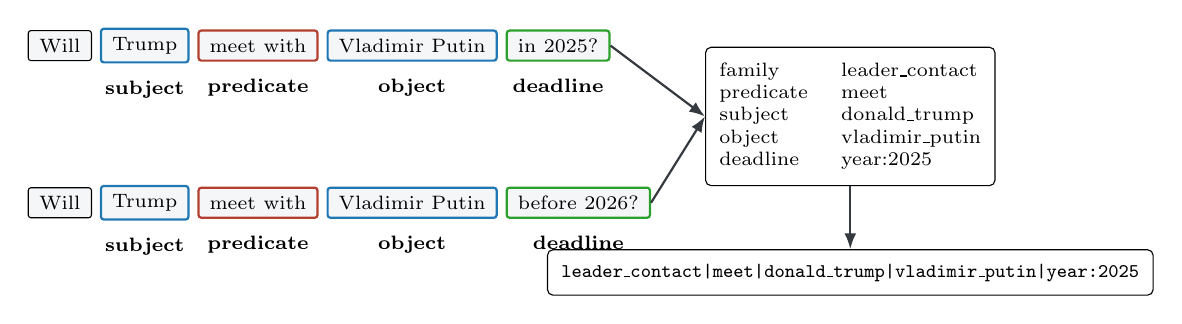
\begin{tikzpicture}[
  token/.style={draw, rounded corners=1pt, fill=softgray, inner xsep=4pt, inner ysep=3pt, font=\scriptsize},
  label/.style={font=\scriptsize\bfseries, align=center},
  key/.style={draw, rounded corners=2pt, fill=white, inner sep=5pt, font=\scriptsize},
  arr/.style={-{Latex[length=2mm]}, thick, darkgray}
]
\node[token] (pm0) {Will};
\node[token, right=1mm of pm0, draw=pmblue, thick] (pm1) {Trump};
\node[token, right=1mm of pm1, draw=riskred, thick] (pm2) {meet with};
\node[token, right=1mm of pm2, draw=pmblue, thick] (pm3) {Vladimir Putin};
\node[token, right=1mm of pm3, draw=kgreen, thick] (pm4) {in 2025?};

\node[label, below=1mm of pm1] {subject};
\node[label, below=1mm of pm2] {predicate};
\node[label, below=1mm of pm3] {object};
\node[label, below=1mm of pm4] {deadline};

\node[token, below=16mm of pm0] (k0) {Will};
\node[token, right=1mm of k0, draw=pmblue, thick] (k1) {Trump};
\node[token, right=1mm of k1, draw=riskred, thick] (k2) {meet with};
\node[token, right=1mm of k2, draw=pmblue, thick] (k3) {Vladimir Putin};
\node[token, right=1mm of k3, draw=kgreen, thick] (k4) {before 2026?};

\node[label, below=1mm of k1] {subject};
\node[label, below=1mm of k2] {predicate};
\node[label, below=1mm of k3] {object};
\node[label, below=1mm of k4] {deadline};

\node[key, right=12mm of pm4, yshift=-9mm] (norm) {
\begin{tabular}{@{}ll@{}}
family & leader\_contact\\
predicate & meet\\
subject & donald\_trump\\
object & vladimir\_putin\\
deadline & year:2025
\end{tabular}
};
\draw[arr] (pm4.east) -- (norm.west);
\draw[arr] (k4.east) -- (norm.west);

\node[key, below=8mm of norm] (ckey) {
\texttt{leader\_contact|meet|donald\_trump|vladimir\_putin|year:2025}
};
\draw[arr] (norm) -- (ckey);
\end{tikzpicture}
\end{center}

\vspace{0.2em}
\begin{columns}[T,onlytextwidth]
\begin{column}{0.48\textwidth}
\textbf{Event-template parsers} claim a title first, setting the market family and the fields that matter.
\end{column}
\begin{column}{0.48\textwidth}
\textbf{Normalization rules} regularize aliases and deadlines: \texttt{Trump} to \texttt{donald\_trump}; \texttt{in 2025} and \texttt{before 2026} to \texttt{year:2025}.
\end{column}
\end{columns}
\end{frame}

\begin{frame}
\small
\begin{columns}[T,onlytextwidth]
\begin{column}{0.32\textwidth}
\begin{itemize}
\tightitem
\item Leader contact
\item Office exit
\item Election
\item Candidate office
\item Generic election winner
\item Sports game
\end{itemize}
\end{column}
\begin{column}{0.32\textwidth}
\begin{itemize}
\tightitem
\item Sports award / prop
\item Sports outcome
\item Fed count
\item Fed decision
\item Crypto threshold
\item Market leader
\end{itemize}
\end{column}
\begin{column}{0.32\textwidth}
\begin{itemize}
\tightitem
\item Geopolitical event
\item Policy action
\item Award winner
\item Media winner
\item Economic threshold
\end{itemize}
\end{column}
\end{columns}
\end{frame}

\begin{frame}
\small
\begin{center}
\begin{table}
\centering
\small
\begin{tabular}{lrrrr}
\toprule
Exchange & Markets & Parsed & Matched & Matched share\\
\midrule
Polymarket & 5,680 & 1,346 & 150 & 2.6\%\\
Kalshi & 8,992 & 1,979 & 149 & 1.7\%\\
\bottomrule
\end{tabular}
\end{table}

\vspace{0.3em}
\begin{table}
\centering
\small
\begin{tabular}{lrr}
\toprule
Exchange & Parsed rate & Volume-weighted parsed rate\\
\midrule
Polymarket & 23.7\% & 88.7\%\\
Kalshi & 22.0\% & 86.6\%\\
\bottomrule
\end{tabular}
\end{table}

\vspace{0.4em}
\smallnote{Strict matching keeps only pairs with the same deterministic \texttt{contract\_key}. Current output: 150 matched rows and 149 unique contract keys.}
\end{center}
\end{frame}

\begin{frame}[plain]
\scriptsize
\centering
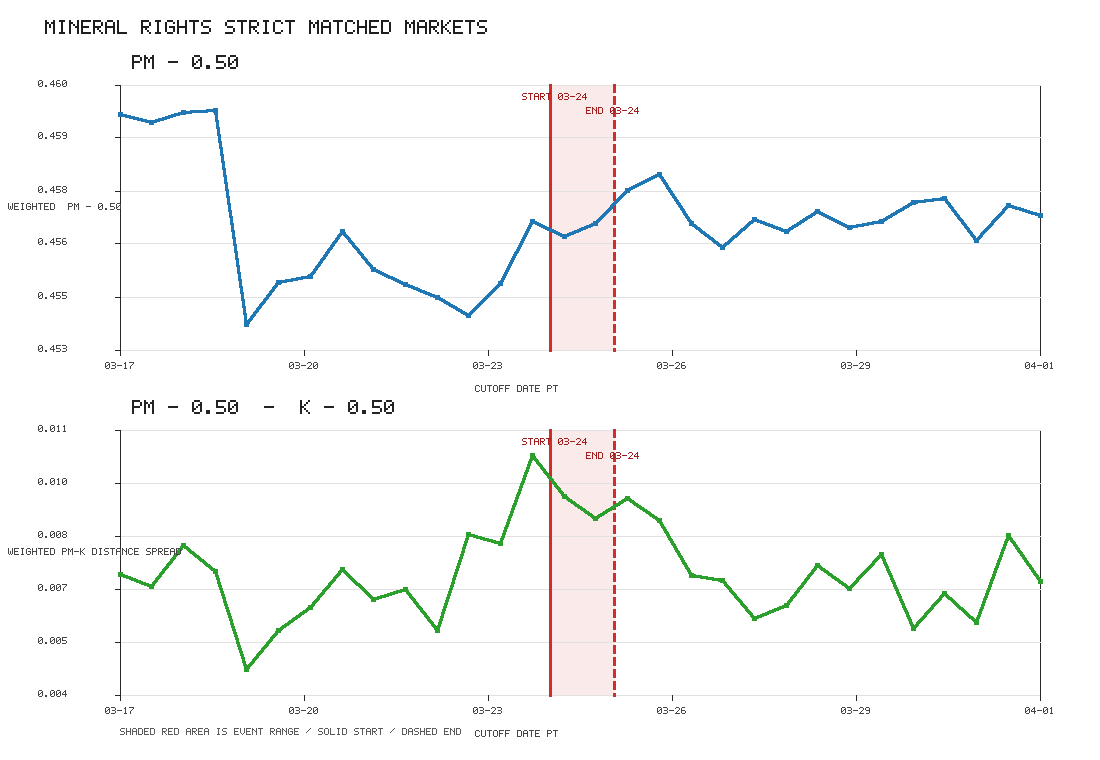
\includegraphics[height=0.82\paperheight,keepaspectratio]{resolution_risk_uma_onchain_attenuation_mineral_rights_timeseries.png}
\end{frame}

\begin{frame}[plain]
\scriptsize
\centering
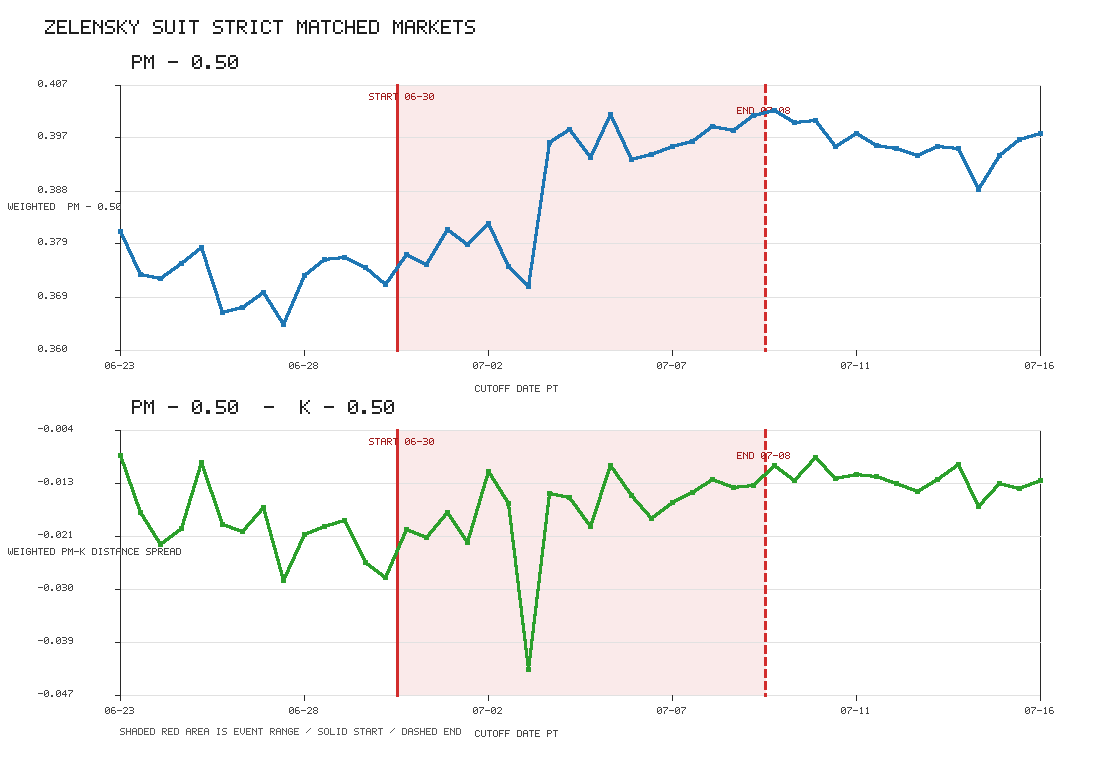
\includegraphics[height=0.82\paperheight,keepaspectratio]{resolution_risk_uma_onchain_attenuation_zelensky_suit_timeseries.png}
\end{frame}

\begin{frame}[plain]
\scriptsize
\centering
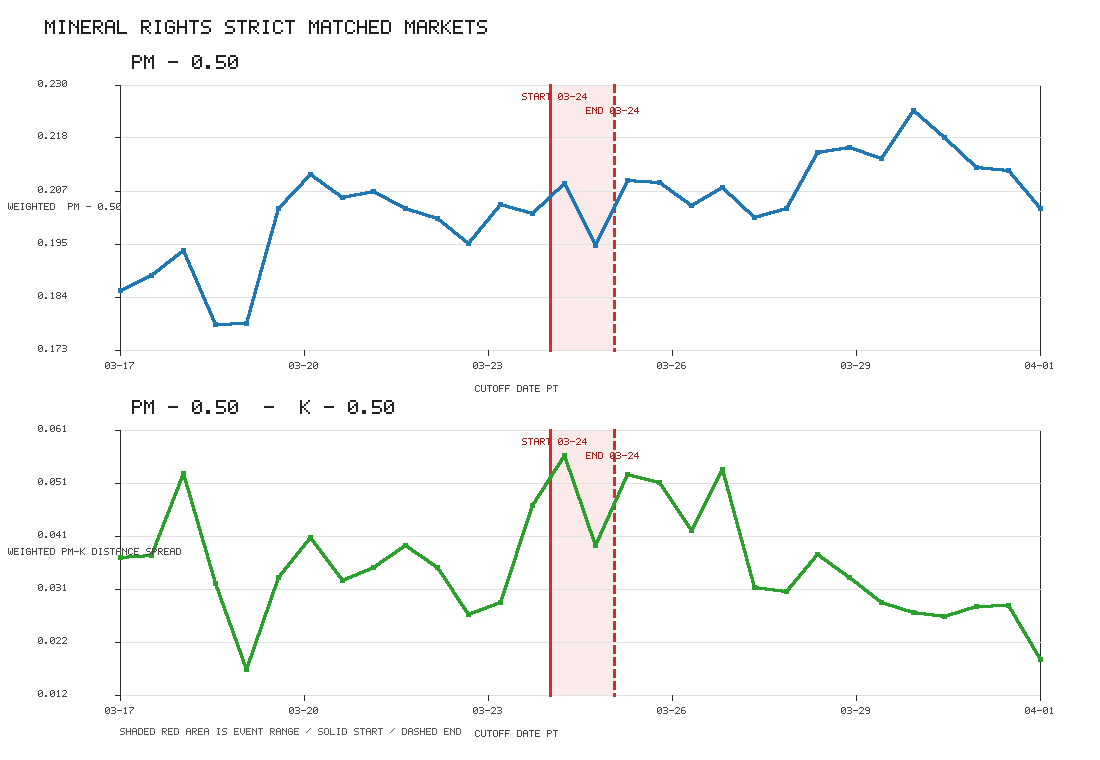
\includegraphics[height=0.82\paperheight,keepaspectratio]{resolution_risk_uma_onchain_similar_types_attenuation_mineral_rights_timeseries.png}
\end{frame}

\begin{frame}[plain]
\scriptsize
\centering
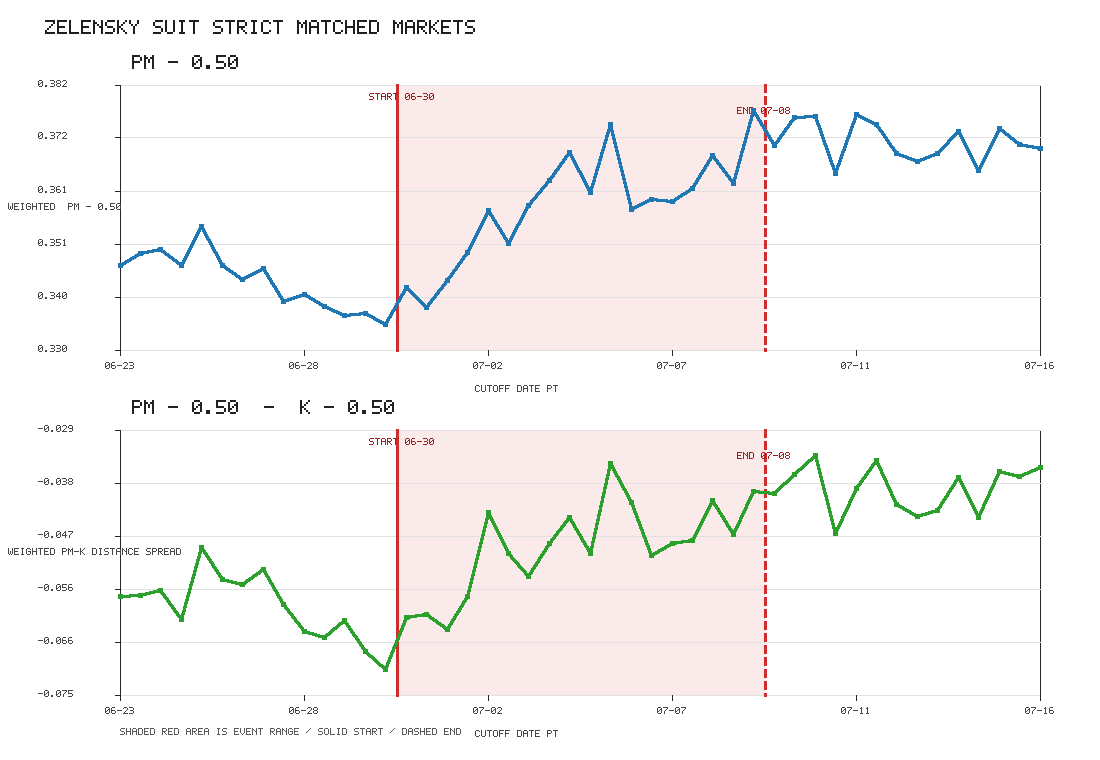
\includegraphics[height=0.82\paperheight,keepaspectratio]{resolution_risk_uma_onchain_similar_types_attenuation_zelensky_suit_timeseries.png}
\end{frame}

\begin{frame}
\scriptsize
\begin{center}
\begin{adjustbox}{max width=\linewidth}
\begin{tabular}{llrrrr}
\toprule
Sample & Outcome & Contracts & Post coef. & SE & t\\
\midrule
Pooled, mineral rights & $|PM-.50|$ & 105 & +0.0010 & 0.0004 & 2.54\\
Pooled, mineral rights & $|PM-.50|-|K-.50|$ & 105 & +0.0003 & 0.0004 & 0.69\\
Pooled, Zelensky suit & $|PM-.50|$ & 57 & +0.0197 & 0.0014 & 14.51\\
Pooled, Zelensky suit & $|PM-.50|-|K-.50|$ & 57 & +0.0047 & 0.0008 & 5.89\\
\addlinespace
Similar, mineral rights & $|PM-.50|$ & 12 & +0.0117 & 0.0031 & 3.80\\
Similar, mineral rights & $|PM-.50|-|K-.50|$ & 12 & +0.0012 & 0.0027 & 0.46\\
Similar, Zelensky suit & $|PM-.50|$ & 19 & +0.0204 & 0.0016 & 12.50\\
Similar, Zelensky suit & $|PM-.50|-|K-.50|$ & 19 & +0.0147 & 0.0013 & 11.24\\
\bottomrule
\end{tabular}
\end{adjustbox}
\end{center}

\vspace{0.4em}
\smallnote{Negative post coefficients would support attenuation toward 50. ``Similar'' is \texttt{uma\_risk\_exposed}: election, office-exit, leader-contact, and policy-action families.}
\end{frame}

\begin{frame}
\small
\begin{columns}[T,onlytextwidth]
\begin{column}{0.49\textwidth}
\textbf{Caveats}
\begin{itemize}
\tightitem
\item PM-volume weights are ex-post.
\item Matched markets are high-precision but not comprehensive.
\item Event windows may blend resolver-risk repricing with unrelated news, liquidity, and price discovery.
\end{itemize}
\end{column}
\begin{column}{0.49\textwidth}
\textbf{Interpreting null or non-attenuation results}
\begin{itemize}
\tightitem
\item UMA failure risk may already have been priced.
\item Traders may not price resolver risk in comparable markets.
\item Failures may be too rare for broad panels to detect.
\item Effects may live only in at-risk subsamples: ambiguous rules, smaller markets, thin liquidity, or terminal windows.
\end{itemize}
\end{column}
\end{columns}
\end{frame}

\end{document}
